\chapter{\label{chap:design}FBase Design}

This chapter will discuss the design of the proposed framework, called FBase. FBase is a framework designed to create a usable ecosystem for the development, distribution, and execution of applications. This chapter will elaborate on the high-level structures within the framework. The implementation considerations and details will be discussed in Chapter~\ref{chap:implementation}. The evaluation of the framework is performed through an experiment (Chapter~\ref{chap:evaluation}).

\section{Overview}

An overview of the architecture of FBase can be found in Figure~\ref{fig:architecture}. It shows the three different layers that make up the framework.

\begin{figure}[h]
	\centering
	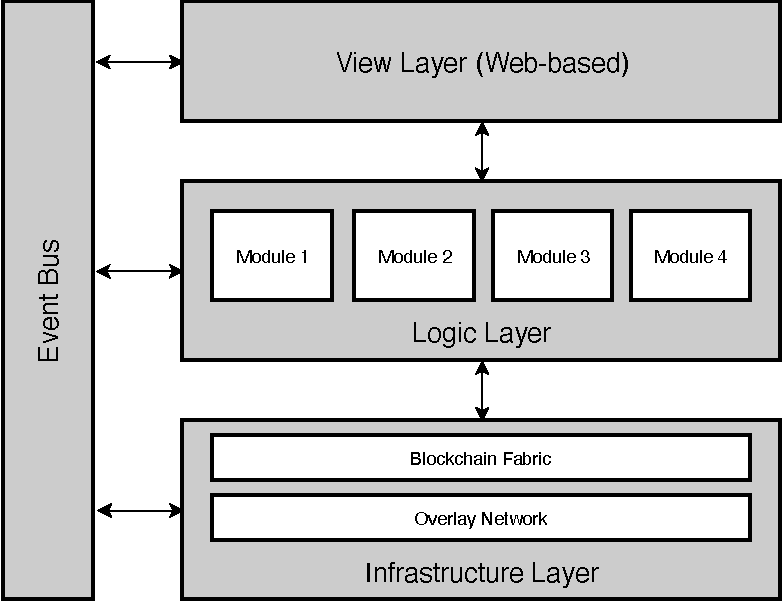
\includegraphics[width=0.5\textwidth]{images/design-architecture.pdf}
	\caption{\label{fig:architecture} The architecture of the FBase framework}
\end{figure}

\begin{itemize}
	\item \textbf{View Layer:}
	The view layer is responsible for the interaction between the user and the logic layer. This layer contains the view components for both the FBase framework and the user applications.
	
	\item \textbf{Logic Layer:} The logic layer is responsible for the execution of the user applications. It provides runtime support through the FBase runtime engine.
	
	\item \textbf{Infrastructure Layer:} The infrastructure layer is responsible for providing services to the FBase framework. These services include database storage, encryption primitives, and network capability. This layer contains the module distribution and overlay network.
\end{itemize}

These layers are connected by a system-wide \textbf{Event Bus} that is used for connecting different parts of the user application. Connecting these components to form the user application can quickly become unmanageable. To prevent this from happening, the FBase framework is built according to the event-driven architecture style. In this style of framework, actions are taken according to events happening in the system. Every component in the framework can trigger events. Creating simple and maintainable logic. Input such as human interaction, network packets, creation of components, and system notifications, trigger these events and cause corresponding actions in other parts of the system. An example of this would be the downloading of a module when a new one is discovered. The event bus is the main method for communications between different layers.

These layers together create the components needed to run and distribute modularized code in a decentralized fashion. The next sections will expand on the components that make up these layers.

\section{Generic Modules}

The FBase framework aims to support as many different use cases of modules as possible. However, to create a single module type that can support any type of interaction and behavior would be infeasible. That would require an interface between modules so generic and complex that it would not satisfy our requirement of a usable system. If such an interface would even be possible to create, it would have a substantial performance penalty because of the abstractions and complexities needed to support such as system.

The method that FBase uses to find a balance between this flexibility and feasibility is a system of four generic modules:

\begin{itemize}
	\item \textbf{View Module:}
	The view module type contains the components that deal with human interaction. This module type is not required for a user application to be functional. The module represents a Graphical User Interface (GUI). 
	
	To meet our goal of having a re-usable ecosystem, these GUIs have to be cross-platform compatible. This cross-platform compatibility enables the view module to be used on any major platform in use today e.g. Windows, macOS, Linux, Android, iOS. To accomplish this, view modules will be created using web technologies. Web technologies were chosen for the FBase user interfaces, as they are one of the only GUI technologies that allow for uniformly looking cross-platform user interfaces. They are becoming the current standard for these kinds of GUIs.
	
	Web technologies also allow for easy decoupling between the view layer and the logic behind it. A view module component consists out of a HTML, CSS, and JavaScript website. This website is run as a standalone component and connects to its logic counterpart through an Application Programming Interface (API). This decouples the user interface part of the user application and allows it to be interchanged. Multiple different GUIs could be offered for the same user application. It also allows GUIs to be created with different purposes that could be run simultaneously. An example of this would be a music visualization plugin.
	
	\item \textbf{Application Module:}
	The application module type is the main module type in the FBase framework. This module type contains the main logic and it is the entry point into the user application. User applications can be either an isolated application on each user's system or a decentralized application that spans across the FBase network overlay.
	
	The logic in the application module type acts as the controller in the Model-View-Controller (MVC) architectural software pattern. Controllers act as an interface between the View module and the Service Module to process all the incoming requests, manipulate data, and interact with the GUI to render the final output.
	
	\item \textbf{Service Module:}
	The service module type provides services to the application module that have common use-cases. These re-usable services should contain the bulk of the code in a user application. Most applications share a significant portion of their functionality with other applications. The service module encapsulates those functionalities to make them more re-usable. A good example of such a service is authentication. Almost every user application needs a form of authentication. Writing a secure and well-structured authentication service is not trivial. When applications can re-use well build services it adds to the usability of the application and ecosystem.
	
	Service modules should be standalone services. They should provide functionality that is not dependent on other parts of the user application. Service modules also maintain their state. This makes sure the complexity of the functionality is encapsulated by the service.
	
	Application modules can also be used as service modules. This can be achieved by marking the module with both types. An example of such a module is a zip code lookup system. Such a system can be used as either a standalone application with a GUI or as a service to another application.
	
	Service modules can also be used to emulate plugin behavior where certain functionality is exchanged by a different one. This is done by changing the service module used in the user application. This ability would be similar to the Strategy software pattern. A use case of this would be changing the algorithm used to calculate trust in a network on runtime. It also allows service to be replaced when security vulnerabilities have been found that are not being fixed.
	
	\item \textbf{Package Module:}
	The package module type is added to make it possible to remove dependencies on existing code repository infrastructure. Many programming languages have a native package manager to house common use code libraries to make it possible to re-use code already used by others. However, these package managers almost all use centralized infrastructure and have many problems of their own e.g. revocability. FBase uses the package module to provide an alternative for these code repositories or act as a back-up.
	
	The Package module contains downloadable code libraries that are made available to the other modules in the system. Examples of use-cases for the package module are validation libraries and database abstraction libraries.
\end{itemize}

\section{Module Discovery and Distribution}

FBase makes use of a decentralized discovery and distribution network for its modules. Current networks for software distribution are often centralized and controlled by a company entity. By making use of a decentralized network,  the possibility of the network being brought down by the company behind it, the government, or the law, can be eliminated. It also allows users to make the FBase network completely self-governing, so the system would be owned by everybody.

\subsection{Identifier and Versioning}
To distinguish different modules from each other, FBase makes use of an identifier. Each module has such an identifier, which is unique in the network. To guarantee this uniqueness a cryptographic asymmetrical key pair is used. An asymmetrical key pair consists out of two keys. One key is the public key to identify the object it represents, in this module. The other key is the private key which can be used to prove the ownership of the represented object. This private key acts as the credential for the author of the module to manage it.

The module identifier consists out of two parts. One part is the previously described public key. The other part is the versioning code. This versioning code is a hash of the entire module code. A hash is a short representation of a piece of data that is calculated in a one-way function. This method is chosen over more conventional versioning code like Semantic Versioning as it makes it significantly harder for malicious actors to spoof the module code corresponding to a version number. Since the hash represents the code.

The complete module identifier format is:
\begin{verbatim}
<public_key>.<module_hash>
\end{verbatim}

New versions of the module have a different module hash and would be a separate entity in the network. Each module also has a timestamp of when the module was created. Together with the module identifier, this allows nodes to pick the most recent version of the module.

When a module wants to introduce breaking changes to the API, a different approach has to be used. Using the current approach for updates with breaking changes could cause dependent modules to break and stop functioning. In FBase when an update includes breaking changes a completely new module has to be created. This means it has a different public key than the previous versions. This approach was chosen because breaking changes are often accompanied by a change in the functionality of the module. FBase represents this change as a new module.

\subsection{Discovery Protocol}

The discovery protocol of FBase relies heavily on crowd-sourcing. It accomplishes this through voting. It is very similar to how code repositories on GitHub gain popularity. The way the discovery protocol works depends on the state of the network. Below different scenarios will be discussed depending on the state of the network. Figure~\ref{fig:discovery-protocol} shows the message flow.

\begin{figure}[h]
	\centering
	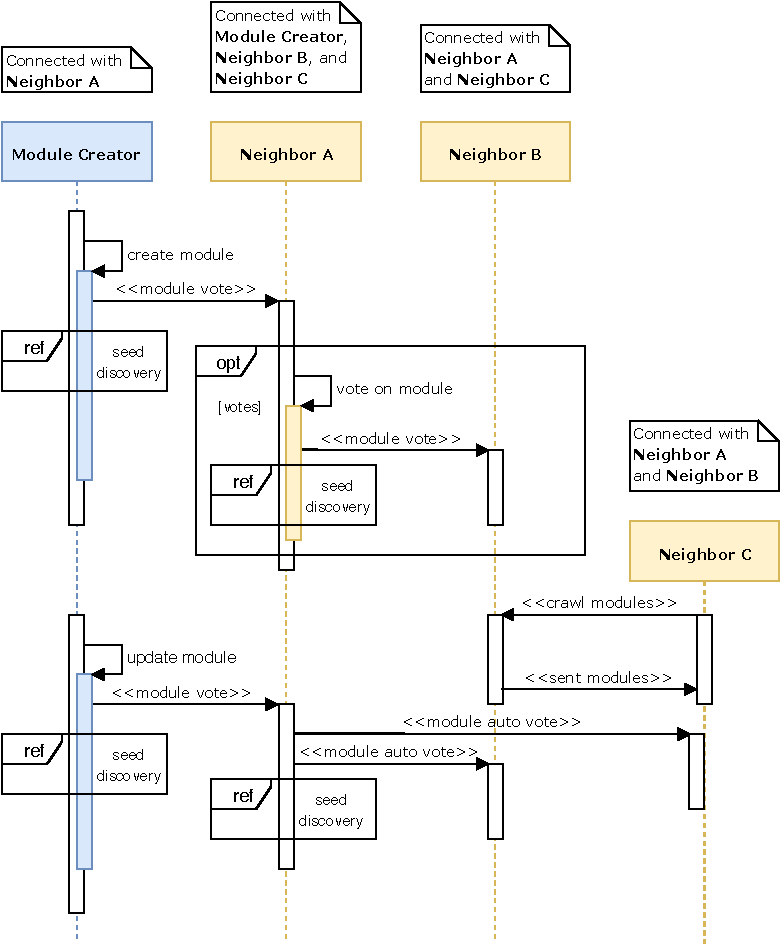
\includegraphics[width=0.75\textwidth]{images/design-discovery-protocol-main.pdf}
	\caption{\label{fig:discovery-protocol} Sequence diagram of discovery protocol.}
\end{figure}

\subsubsection{\textbf{Scenario 1: New Module}}

When a new module is created the network is not aware of this. To make it possible for other nodes to discover this new module, the author will automatically cast its vote. This vote is stored on a blockchain and includes the public key of the voting node, a voting timestamp, and a module manifest. The module manifest contains the module identifier, module timestamp, and a description. The block representing this vote is sent to all connected neighbors in the FBase overlay network of the current node. 

To give modules a better chance at discovery, FBase makes use of a mechanism called \textbf{Seed Discovery} (as shown in Figure~\ref{fig:seed-discovery}). In this mechanism, 10 seed messages will each be sent through 10 intermediate nodes to reach their \textbf{Seed Point}. At each hop, these nodes select one of its connected neighbors at random, excluding the neighbor where the message originated from. The \textbf{Seed Point} will discover the module and make a simulated vote, called \textbf{Seed Vote}, that also informs its connected neighbors. This approach creates multiple different starting points from which modules can be discovered. This increases the possibility of a module to be discovered on a larger scale.

At the end of this scenario, the author and the 10 \textbf{Seed Points}, and their connected neighboring nodes know about the new module.

\begin{figure}[h]
	\centering
	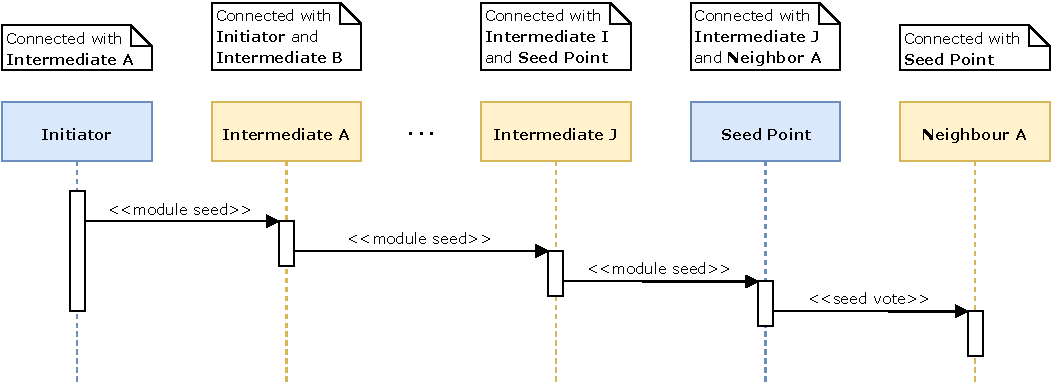
\includegraphics[width=1\textwidth]{images/design-discovery-protocol-seed.pdf}
	\caption{\label{fig:seed-discovery} Seed discovery mechanism.}
\end{figure}

\newpage

\subsubsection{\textbf{Scenario 2: Upvoting}}

When users discover new modules they can inspect the module and determine if they want to upvote it. When the user determines they do not want to vote on the module, the spreading is terminated at the current node. When they do want to vote on the module, the module information is distributed in the same way as in Scenario 1. This is done to promote the spreading of quality modules and hinder the spreading of bad quality ones. 

\subsubsection{\textbf{Scenario 3: Updated Module}}

When a module is updated a new version has to be discovered by the network. To make sure critical updates are discovered as fast as possible, nodes automatically vote on updated nodes when they have voted on the previous versions. This fast updating is critical to prevent security vulnerabilities from persisting in code bases longer than necessary. In a framework designed around re-usable code, security vulnerabilities are a significant problem since many different applications rely on the same pieces of code. One vulnerability can affect many different applications. 

\subsubsection{\textbf{Scenario 4: New Node}}

The previous scenarios do not solve the bootstrapping problem, where nodes that are new in the network do not have any information about modules before the node joined the network. The node will only discover modules voted on by its connected neighbors after it joined the network.

To bootstrap new users, the node crawls the blockchain of its connected neighbors. During this crawling, it fetches the modules that have been discovered by these neighbors and stores them in its own blockchain.

\subsubsection{\textbf{Performance}}

The performance of the discovery protocol is determined by multiple factors.

One of these factors is the number of connected nodes each node has. This controls the speed at which modules can spread through the network. Making this value too low creates a scenario where modules have a difficult time being discovered when just created. Making this value too big could flood the network with (malicious) modules and create a Distributed Denial Of Service (DDOS) attack.

Another of these factors is the active involvement of users of the system. When users don't actively participate in the voting process, it makes it considerably harder for modules to be discovered by the entire network.

A third factor is how capable users are in determining the quality of modules. When users vote on almost every item, it would flood the network. Since each user would send a message to all its connected neighbors for every module it knows about. 

By making use of an event-driven discovery protocol, FBase tries to find a balance between the speed at which modules can spread through the network and preventing a flood.

\subsection{Distribution}

When nodes have discovered modules, the module code has to be distributed to them. To meet the requirements that where determined in Chapter 2, the distribution mechanism has to be decentralized.

By making the distribution mechanism decentralized it allows the network to operate without a central point of failure. Another benefit of this approach is that the load of storing and distributing the module code is spread across the users of the network. When nodes download a module it increases the availability of that module within the network. This means that modules that are more popular and will be downloaded more often, have a higher availability to scale with this. Modules that are less popular will have a lower availability to correspond with the demand.

Each module must have a minimum availability to make sure that every module that is discovered is also available to download. To make sure this happens the author of the module always keeps a local copy of the module. Besides this copy, the Random Discovery mechanism will make sure that a minimum number of other nodes also have a copy to prevent a problem when the original author is offline. When a Random Discovery message is received that node automatically downloads the module to increase the availability of it temporarily.

If a node has a copy of a module that it has not used for a while this module is deleted from that node to keep the network lean and fit.
% Find different module versions by module identifier

\subsection{System Strategies}

Since the framework deals with untrusted executable user code, the framework provides different strategies that the user can select from to protect their system against possible threats from running this code.

%\subsection{Download and Retention Strategy}

The framework allows the user to configure and replace the download and retention strategy. This strategy is responsible for choosing which components get downloaded and how long they are kept on the system. For the distribution of components, it is necessary to download packages that might not be used by the host system itself but are solely for the intent of distributing. Some users might want to take a different approach to accomplish this. The framework addresses this by allowing parts of its code to be replaced by other components written by a third-party or by the user itself.

\section{Blockchain Organizational Principles}

FBase requires a blockchain that can store tamper-proof and accurate data records.
We now explore three common blockchain structures, displayed in Figure~\ref{fig:blockchain_structures}.

\begin{figure*}[th!]
	\centering
	\begin{subfigure}[t]{.3\textwidth}
		\centering
		\captionsetup{width=.9\linewidth}
		\raisebox{4mm}{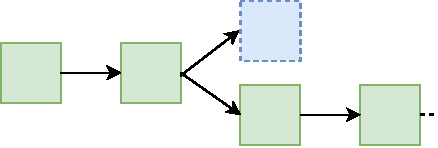
\includegraphics[width=\linewidth]{images/design-blockchain-single.pdf}}
		\caption{Linear ledger (Ethereum).}
		\label{fig:blockchain_single}
	\end{subfigure}\hfill%
	\begin{subfigure}[t]{.3\textwidth}
		\centering
		\captionsetup{width=.9\linewidth}
		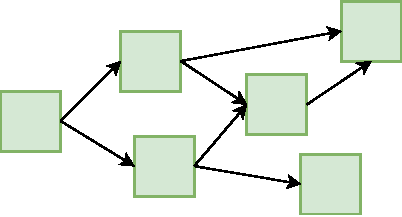
\includegraphics[width=\linewidth]{images/design-blockchain-dag.pdf}
		\caption{DAG ledger (IOTA).}
		\label{fig:blockchain_dag}
	\end{subfigure}\hfill%
	\begin{subfigure}[t]{.3\textwidth}
		\centering
		\captionsetup{width=.9\linewidth}
		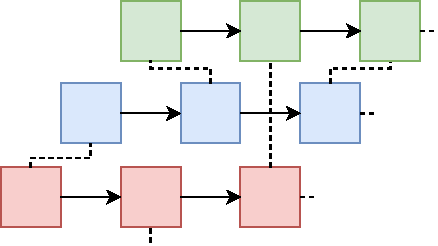
\includegraphics[width=\linewidth]{images/design-blockchain-pairwise.pdf}
		\caption{Pairwise ledger (Nano).}
		\label{fig:blockchain_pairwise}
	\end{subfigure}%
	\caption{Three different structures of distributed blockchain ledgers. Each arrow points to the subsequent block in the chain.}
	\label{fig:blockchain_structures}
\end{figure*}

\subsubsection{\textbf{Linear ledger:}} 
Figure~\ref{fig:blockchain_single} shows the linear blockchain ledger used by Ethereum.
The fundamental property of this ledger is that at least a majority of users agree on the exact sequence of transactions.
A global consensus mechanism like Proof-of-Work or Proof-of-Stake prevents the double-spend attack where a malicious user intentionally creates a fork of their chain~\cite{vukolic2015quest}.
While providing a high level of consistency, the transaction throughput of these ledgers is often not high enough to facilitate record creation and modification by millions of users.
This motivates us to consider different blockchain structures for FBase.

\subsubsection{\textbf{DAG ledger:}} 
Another blockchain structure is the Directed Acyclic Graph (DAG) ledger, where each block can be referenced by multiple other blocks.
This ledger structure, shown in Figure~\ref{fig:blockchain_dag}, is adopted by blockchain platforms like IOTA and Dagcoin~\cite{popov2018tangle}~\cite{lerner2015dagcoin}.
IOTA is optimized for micro-payments within Internet-of-Things, and Dagcoin advertises itself as data storage for arbitrary data (e.g., documents or ownership records).
Since these ledgers allow for different consensus mechanisms, transaction throughput is often superior compared to that of linear ledgers.
However, they usually do not have the same consistency guarantees.
While these ledger structures are more suitable for data storage, we consider current implementations unfit for the storage of votes.
The reason is that they either rely on a centralized coordinator (IOTA) or a fixed group of witness nodes (Dagcoin).
Instead, our goal is to devise an infrastructure without any authority with leveraged permission.

\subsubsection{\textbf{Pairwise Ledger:}}
A third blockchain structure we consider is the pairwise distributed ledger.
The key property of this ledger, given in Figure~\ref{fig:blockchain_pairwise}, is that each user maintains and grows their individual chain with transactions.
Each block holds exactly one transaction and optionally contains a (hash) pointer to a transaction in the individual chain of another user.
Blockchain fabrics like R3 Corda, Nano, and TrustChain, use pairwise ledgers as their underlying data structure~\cite{otte2017trustchain}~\cite{lemahieu2017raiblocks}~\cite{brown2017introducing}.
These platforms address the double-spending attack either by a trusted notary (Corda), a weighted voting system (Nano) or by guaranteed eventual consistency (TrustChain).
In general, they provide superior scalability compared to linear ledgers as used by Bitcoin and Ethereum but lack global consensus.

We strongly believe that the pairwise distributed ledger is a suitable data structure to store voting records as transactions.
Compared to linear and DAG ledgers, only data that the user is interested in is stored on that user's host.
Pairwise distributed ledgers enable selective queries of data stored on the chains of other members, without the need for full data replication across the network.
In FBase, each individual ledger stores all data associated with the actions taken by the user of that node, in a tamper-proof manner, and without global agreement.

\section{Trust}

Since this framework that is highly dependent on re-usable code, it is important that the user running the application can trust all its parts.

\subsection{Verifiable Modules}

To determine if a module can be trusted, the user should know what the module is supposed to do and what the module is actually doing. This is an important part of the voting protocol. Therefore, all modules should be verifiable. This means that the code in the module should be identical to the one the author controls and be open for inspection.

To accomplish this, every module should be cryptographically signed by the author. This digital signature can be verified by using the public key in the module identifier. This makes it impossible for malicious users to distribute a different version of the module. Only users who have access to the cryptographic key pair of the module can distribute new versions of the module.

The code base of a module must also be publicly available for all users of the network to inspect. This is achieved by distributing the code base openly through the network.

\subsection{Identity Profiles}

In peer-to-peer systems, each peer in an overlay has to have an identity. This identity determines the trust and association within and across overlays. This identity can be shared between different overlays or each overlay can use its own identity. If two overlays use the same identity, one overlay can benefit from the built-up trust and reputation of another overlay. However, actions performed by one overlay can also have a negative trust impact on the other overlay. To allow applications to choose between having a shared identity, having its own identity, or having a pseudo-random identity,  the framework provides a configuration option in the module configuration file to select what kind of identity profile is preferred.

\subsection{Verified Identities}
\label{subsec:strong_identities}
To further improve the trustworthiness of modules, users can optionally verify their digital identity.
A verified identity is uniquely linked to a real-world entity.
Software built on FBase can give preferential treatment to module authors that have verified their identity.

Identity verification can be done with an attestation given by a trusted third party like the government or a notary.
Enforcing strong, long-lived identities in FBase is comparable with account validation that many centralized platforms use (e.g., the verification of a phone number).
The requirement for verified identities addresses the Sybil Attack, where an adversary assumes multiple fake identities to influence or subvert the network~\cite{douceur2002sybil}.

Two solutions are proposed to achieve trustworthy importation of data: \textit{challenges} and \textit{TLS auditing}.

The first solution is to pose a challenge where the user importing the data, proves that they have control over this data.
For example, when importing data from GitHub, we can require a public identifier (e.g., a public key) of the developer to be part of the \enquote{bio} profile field.
This information can then be verified for correctness by other users who query the public GitHub API.
Users who verify data are called \emph{witnesses}.
While this is a basic mechanism to ensure the accuracy of imported data, it heavily depends on the availability of a public API.

The second solution is TLS auditing~\cite{tlsnotary2014whitepaper}.
The key idea is to proxy a TLS connection through a random witness, which then verifies and signs the data after the TLS connection terminates.
When the TLS session finishes, the client gives the witness the private key used to decrypt HTTPS responses from the web service.
Note that this way the witness is not able to decrypt the request made to the web service, which likely includes credentials or access tokens.
The role of a witness can either be fulfilled by other entities in the network, or by a trusted notary service.
Depending on the significance of data being imported, multiple witnesses can be used for this.
Compared to challenges, TLS auditing works when access to a public API is absent but is more advanced.
%Our lab has implemented an advanced TLS auditing mechanism, which is currently under a security audit.

\section{Runtime Support}

Once modules are discovered and distributed to the nodes in the network, they will be used to run in applications on the system. To accommodate this runtime support is necessary.

%\subsection{Dynamic loading}
%To increase the usability of the platform, all modules should be dynamically loaded into the execution environment.

\subsection{Module Interconnect Mechanisms}

To combine the different modules into the user application the module interconnect mechanism is used. This mechanism uses a top-down search approach. When a module searches for a dependency, it sends a message on the event bus specifying the module type and name.

View modules can load Application modules. Application modules can load Service Modules and Package modules. Service modules can load Package modules. Package modules can load other package modules.

When the lower module receives the event for itself, it registers itself with the higher module.
%Modules search for dependencies downwards
%View layer triggers search for logic layer
%Logic layer triggers search for other logic layer
%After search they register with the higher module
%Module abstracts classes for registration mechanism

%Key value store for storing settings in dependent modules

\subsubsection{\textbf{View Module}}
When a new view component is added to the system, it needs to know how to connect to the logic component of the application. It does this by triggering an event on the event bus, specific for the type of application it belongs to, indicating it is requesting an endpoint address. The logic component is subscribed to this event. Its registered handler will return the REST API endpoint address to the view component through the event bus.

To define a view component, a special file has to be created: manifest.json. This definition file stores the attributes and the settings of the view component. Attributes of the file include name, version, and app-tag (Application tag used for hooking on to the logic component). Each view component also needs to have a directory named public which contains the index.html file. 

%An example structure can be found below.
%\begin{itemize}
%	\item manifest.json
%	\item public \begin{itemize}
%		\item index.html
%		\item Other HTML/CSS/javascript resources
%	\end{itemize}
%\end{itemize}

%\subsection{Seamless Upgrading}

\subsection{Isolated Execution}

Since all distributed components have to be executed on the host system for them to function, it can pose a security risk by running untrusted user code. To minimize the risk that this poses, the framework allows components to be run inside of an isolated execution environment using Docker. When this method is used an execution environment is set up inside of the docker engine and the code will be mounted inside of this container. This container will then be able to run the code in isolation. This method, however, will prevent other applications running on the system from communication to it. It does allow the view layer to communicate with the isolated components since this makes use of network sockets.